\hypertarget{group__usecase1}{}\section{Use case 1}
\label{group__usecase1}\index{Use case 1@{Use case 1}}
Collaboration diagram for Use case 1\+:\nopagebreak
\begin{figure}[H]
\begin{center}
\leavevmode
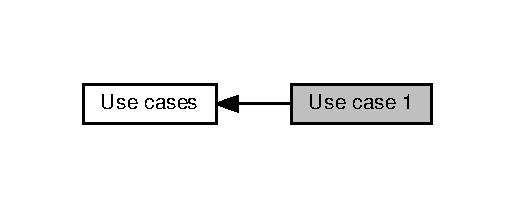
\includegraphics[width=247pt]{group__usecase1}
\end{center}
\end{figure}



\begin{DoxyCode}
\textcolor{preprocessor}{#include "bitmap.cuh"}
\textcolor{preprocessor}{#include "geometryLoader.cuh"}
\textcolor{keyword}{template} <> \textcolor{keyword}{const} \hyperlink{class_square_matrix4}{SquareMatrix4f} SquareMatrix4f::Identity = 
      \hyperlink{class_square_matrix4}{SquareMatrix4f}();
\textcolor{keywordtype}{int} main(\textcolor{keywordtype}{int} argc, \textcolor{keywordtype}{char} **argv)\{
    \hyperlink{class_vec3}{Vec3f} boundingPlaneNormals[] = \{
            \hyperlink{class_vec3}{Vec3f}(1, 0, 0),
            \hyperlink{class_vec3}{Vec3f}(0, 1, 0),
            \hyperlink{class_vec3}{Vec3f}(0, 0, 1),
            \hyperlink{class_vec3}{Vec3f}( sqrtf(3) / 3.f,  sqrtf(3) / 3.f, sqrtf(3) / 3.f),
            \hyperlink{class_vec3}{Vec3f}(-sqrtf(3) / 3.f,  sqrtf(3) / 3.f, sqrtf(3) / 3.f),
            \hyperlink{class_vec3}{Vec3f}(-sqrtf(3) / 3.f, -sqrtf(3) / 3.f, sqrtf(3) / 3.f),
            \hyperlink{class_vec3}{Vec3f}( sqrtf(3) / 3.f, -sqrtf(3) / 3.f, sqrtf(3) / 3.f) \};
        \textcolor{comment}{//Create the camera settings}
        \hyperlink{struct_camera}{Camera} camera;
        \textcolor{comment}{//set up screen width and heght, field of view and scale}
        camera.\hyperlink{struct_camera_ab0cbf1b102afdeb285ef2be271d1701c}{resolution}(960, 540, 36.87, 0.5);
        \textcolor{comment}{//create a transformation pipeline. One can set an identity matrix to not make any changes.}
        std::unique\_ptr<Pipeline> pipeline( \textcolor{keyword}{new} \hyperlink{class_mesh_transformation}{MeshTransformation}());
        pipeline->translate( make\_float3(0,0,10));
        pipeline->scale( make\_float3(1,1,1) );
        \textcolor{comment}{//Usually it's appropriate to perform the same transformation with both camera origin and camera
       direction.}
        camera.modelDir = pipeline->transform() * defaultCameraMatrix.inverse();
        camera.modelOrig = camera.modelDir;
        \textcolor{comment}{//set lights}
        std::vector<ILight> lights;
        std::unique\_ptr<Pipeline> light\_pipeline( \textcolor{keyword}{new} \hyperlink{class_mesh_transformation}{MeshTransformation}());
        \hyperlink{class_square_matrix4}{SquareMatrix4f} light\_model(0.95292, 0.289503, 0.0901785, 0,
                      -0.0960954, 0.5704, -0.815727, 0,
                      -0.287593, 0.768656, 0.571365, 0,
                    0, 0, 0, 1);
        \textcolor{comment}{//create 2 distant light sources}
        light\_pipeline->translate( make\_float3(0,0,5));
        lights.push\_back( \hyperlink{class_i_light}{ILight}( light\_model, \hyperlink{class_vec3}{Vec3f}(1, 1, 1), 1.0f, DISTANT\_LIGHT) );
        lights.push\_back( \hyperlink{class_i_light}{ILight}( light\_pipeline->transform()*light\_model, 
      \hyperlink{class_vec3}{Vec3f}(1, 1, 1), 1.0f, DISTANT\_LIGHT) );

        \textcolor{comment}{//create an instance of the specular plane settings}
        \hyperlink{struct_appearence}{Appearence} plane(0.8);
        \hyperlink{struct_appearence}{Appearence} sphere( \hyperlink{class_vec3}{Vec3f}(1,0, 0), 0.8f, 0.2f, 4.f, \textcolor{stringliteral}{"none"} );
        plane.setObjectColor(\hyperlink{class_vec3}{Vec3f}(0.5));
        plane.setTextureColor(\hyperlink{class_vec3}{Vec3f}(0.5));
        sphere.setTextureColor(\hyperlink{class_vec3}{Vec3f}(1, 0, 0 ) );
        \textcolor{comment}{// to get it into the engine one should pack it into stl vector}
        std::vector<Appearence>  appearences;
        appearences.push\_back(plane);
        appearences.push\_back(sphere);
        \textcolor{comment}{//use interface HostObject to store instances of scene geometries}
        std::vector<std::unique\_ptr<HostObject>> host\_obj;
        host\_obj.push\_back(std::unique\_ptr<HostObject>(\textcolor{keyword}{new} \hyperlink{class_plane}{Plane}( \hyperlink{class_vec3}{Vec3f}(-20, 0, 20), 
      \hyperlink{class_vec3}{Vec3f}(20, 0, 20), \hyperlink{class_vec3}{Vec3f}(20, 0, -25) )));

        host\_obj.push\_back(std::unique\_ptr<HostObject>(\textcolor{keyword}{new} \hyperlink{class_sphere}{Sphere}( \hyperlink{class_vec3}{Vec3f}(0, 10, -10), 3.0f, 
      boundingPlaneNormals )   ));
        \textcolor{comment}{//Main step. Creation of the geometry manager.}
        \hyperlink{class_geometry_loader}{GeometryLoader<Mesh, Boundaries>} loader(host\_obj, lights, 
      appearences);
        \textcolor{comment}{//Display support.}
        \hyperlink{class_bitmap_maker}{BitmapMaker< GeometryLoader<Mesh, Boundaries>} > bitmap
      (camera.width(), camera.height());
        \textcolor{keywordflow}{try}\{
            bitmap.display(camera, loader);
        \}\textcolor{keywordflow}{catch}(\textcolor{keyword}{const} std::exception& e)\{
            std::cout<<e.what()<<std::endl;
        \}

        \textcolor{keywordflow}{return} 0;
\}
\end{DoxyCode}
 